%% =====================================================================
%%  Savana -- paper skeleton targeting USENIX Security '27
%%
%%  Build (Overleaf): compiler = pdfLaTeX, main document = main.tex,
%%  bibliography = BibTeX.  Place the official USENIX style file
%%  `usenix-2020-09.sty` (from the USENIX author-resources page) next to
%%  this file; until it is present the fallback style `usenix-fallback.sty`
%%  is used so that the project compiles.  See README.md.
%%
%%  Status: design/implementation sections are drafted from the code at
%%  commit bee2ed3 (2026-09-02).  Section 9 (Evaluation) is a skeleton:
%%  research questions, setup and table shells are in place, all numbers
%%  are marked TBD.  Search for "TODO" before submission.
%% =====================================================================
\documentclass[letterpaper,twocolumn,10pt]{article}

\IfFileExists{usenix-2020-09.sty}%
  {\usepackage{usenix-2020-09}}%
  {\usepackage{usenix-fallback}}

\usepackage[T1]{fontenc}
\usepackage[utf8]{inputenc}
\usepackage{amsmath,amssymb}
\usepackage{booktabs}
\usepackage{array}
\usepackage{tabularx}
\usepackage{multirow}
\usepackage{graphicx}
\usepackage{xcolor}
\usepackage{enumitem}
\usepackage{listings}
\usepackage{tikz}
\usetikzlibrary{arrows.meta,positioning,fit,calc,shapes.geometric}
\usepackage{url}
\usepackage[hidelinks]{hyperref}

% ---------------------------------------------------------------------
% Submission switches
% ---------------------------------------------------------------------
\newif\ifanonymous
\anonymoustrue            % USENIX Security submissions are double-blind

% ---------------------------------------------------------------------
% Macros
% ---------------------------------------------------------------------
\newcommand{\sys}{Savana}
\newcommand{\code}[1]{\texttt{\detokenize{#1}}}
\newcommand{\todo}[1]{{\color{red}\textbf{[TODO: #1]}}}
\newcommand{\tbd}{{\color{red}TBD}}
\newcommand{\pending}[1]{{\color{blue!60!black}\textit{#1}}}
\newcommand{\lbl}[4]{\ensuremath{\langle #1,\,#2,\,#3,\,#4\rangle}}
\newcommand{\READ}{\textsc{read}}
\newcommand{\SEND}{\textsc{send}}
\newcommand{\integ}{\mathit{int}}
\newcommand{\conf}{\mathit{conf}}
\newcommand{\readers}{\mathit{readers}}
\newcommand{\effects}{\mathit{effects}}
\newcommand{\join}{\sqcup}

\lstdefinelanguage{Rust}{
  morekeywords={fn,let,match,pub,const,impl,enum,struct,Some,None,Ok,Err,return,if,else,for,in,mut,use,mod,trait,where,as,ref,self,Self},
  sensitive=true,
  morecomment=[l]{//},
  morecomment=[s]{/*}{*/},
  morestring=[b]",
}
\lstset{
  basicstyle=\ttfamily\scriptsize,
  columns=fullflexible,
  keepspaces=true,
  breaklines=true,
  frame=single,
  framerule=0.3pt,
  xleftmargin=4pt,
  xrightmargin=4pt,
  aboveskip=6pt,
  belowskip=6pt,
  language=Rust,
  keywordstyle=\bfseries,
  commentstyle=\color{black!55},
}

\setlist{nosep,leftmargin=*}

% ---------------------------------------------------------------------
\begin{document}

\date{}

\title{\Large \bf \sys{}: An Information-Flow Kernel that Governs Disclosure and Effects\\for Language-Model Agents}

\ifanonymous
\author{
  {\rm Anonymous Author(s)}\\
  Submission to USENIX Security '27
}
\else
\author{
  {\rm Feiyun Zhao}\\
  \todo{affiliation}
}
\fi

\maketitle

% =====================================================================
\begin{abstract}
Systems that let a large language model (LLM) act on a user's behalf have
an architectural security problem: the model is at once the component that
interprets untrusted content and the component that decides what to do.
Prompt injection is therefore not a defect to be patched but a consequence
of where the security boundary sits. Defenses that harden instructions,
classify inputs, or sandbox tools keep the boundary at or inside the model
and fail against an adversary who controls the model's input.

We present \sys{}, a security kernel that moves the boundary out of the
model. The model is an untrusted \emph{proposer}: it may request actions but
holds no capability to perform them. Every value in the kernel carries a
four-dimension label \lbl{\integ}{\conf}{\readers}{\effects}; derivation
only narrows a value's audience, and the invariant
``externally-untrusted integrity implies effects~$\subseteq\{\READ\}$'' is
re-established after every join so that authority cannot be laundered by
combination. The \emph{only} operation that widens a value's audience is a
declassification transition drawn from a closed set of five, each
authorized by a signed, hash-chained rule set pinned by the deployment
manifest, verified by an in-kernel deterministic content gate whose evidence
is computed by the gate rather than asserted by its caller, recorded as an
immutable provenance node, and---for the two transitions that hand a value
to one recipient---bound to that recipient's exact identity. A signed
policy supply chain determines what is \emph{possible}; runtime gates,
single-use human-approval settlements and a journal-before-effect dispatch
pipeline determine what is \emph{permitted} in each instance.

\sys{} is implemented in about 296K lines of Rust as five mutually
authenticated daemons with sandboxed one-job workers, together with a client
SDK and a production integration into an existing agent framework. Beyond
values, it withholds plan \emph{shape} and user \emph{intent} from a remote
planning model, and admits user-registered connectors through a hash-chained
registry whose tier is a capability ceiling. We report the design, the
principles we extracted from defects found while building it, and the
properties the implementation enforces mechanically. \todo{one sentence of
headline evaluation results once Section~\ref{sec:eval} is complete.}
\end{abstract}

% =====================================================================
\section{Introduction}
\label{sec:intro}

An agentic system embeds a language model in a loop with tools: the model
reads content, chooses an action, and the surrounding system performs it.
In every realistic deployment the content is attacker-influenced---web
pages, documents, e-mail, and the results of earlier tool calls---and it
arrives in the same channel as the user's instructions. The model has no
reliable way to tell them apart. This is prompt injection~\cite{perez2022ignore,greshake2023}, and several years of
mitigation research~\cite{wallace2024hierarchy,hines2024spotlighting,chen2025struq,chen2025secalign,liu2024formalizing}
have not produced a defense that holds against an adaptive adversary, because
the mitigations operate \emph{inside} the abstraction that creates the
problem.

Systems security has long known the shape of the answer. A component that
cannot be trusted to make a decision must not hold the authority to enact
it~\cite{saltzer1975,dennis1966,miller2006robust}. Capability confinement and
information-flow control (IFC)~\cite{denning1976,myers1997,efstathopoulos2005,zeldovich2006,krohn2007}
are the classical mechanisms, and recent work---most prominently the CaMeL
line~\cite{debenedetti2025camel}---has shown that they apply naturally to LLM
agents by separating the control plane from the data plane and attaching
capabilities to values. That work established feasibility at prototype
scale.

The gap this paper addresses is the distance between that result and a
system one can operate. A prototype may assume its policy is correct and
present; a real system must obtain policy over a signed, revocable,
hash-chained supply chain and behave sanely when policy is absent, stale, or
rolled back. A prototype may assume it does not crash; a real system must
journal before it acts and must be able to say, honestly, that a value came
from an action whose outcome it only learned after a restart. A prototype
may assume its trusted components are trustworthy; a real system must
assume that the executor, the approval service, the network, and the user's
own browser are separately compromisable and must bind each interaction
cryptographically. And a prototype may protect data \emph{values} while
leaking the \emph{shape} of the user's plan and the \emph{intent} behind it
to whichever model does the planning.

\sys{} is our attempt to close that gap. Its central design commitment is
that the model \emph{proposes} and the kernel \emph{disposes}: the agent
process holds no capability at all---it cannot read a stored value, call a
tool, or release data---and can only send requests to a kernel that decides,
over labeled evidence the model cannot forge, what to return.

\paragraph{Contributions.}
\begin{enumerate}[label=\textbf{C\arabic*}]
\item \textbf{A four-dimension label model with an enforced untrusted-effect
  ceiling} (\S\ref{sec:labels}). We show that the invariant
  $\integ=\textsf{ExternalUntrusted} \Rightarrow \effects\subseteq\{\READ\}$,
  applied at construction, at derivation, \emph{and again after every join},
  is what prevents \emph{effect laundering}: the acquisition of authority by
  combining attacker-controlled content with a trusted value.
\item \textbf{Declassification as the system's only widening operation,
  governed end to end} (\S\ref{sec:declass}). Derivation intersects reader
  sets, so audience growth requires one of five explicit transitions. Each
  is authorized by a signed rule set rooted in the operational trust roots
  and pinned by the deployment manifest, verified by a deterministic content
  gate that runs \emph{inside} the record constructor, subject to a
  three-valued handoff judgment that reads the confidentiality and reader
  dimensions, and---for executor and egress handoffs---bound to the exact
  recipient identity. All five transitions are on the production path.
\item \textbf{A signed policy supply chain and a journal-before-effect action
  pipeline} (\S\ref{sec:authority}). Hash-chained trust-root sets with
  per-purpose members, canonical re-encode equality on every signed object,
  two-ceremony human approval bound to signed single-use settlements, an
  atomic effect-preparation transaction, an executor journal that is the
  durable truth at the external-byte boundary, and a provenance source kind
  that names values recovered after a crash.
\item \textbf{Privacy beyond values} (\S\ref{sec:beyond}). A three-stage
  planning pipeline in which a remote planner sees only a de-semanticized
  structural graph with fresh node identifiers, a deterministic (never
  model-based) decoder maps plans back to authorized tools, and intent
  exposure is a single explicit, fail-safe-to-private knob; plus a
  hash-chained connector registry in which a connector's tier is a
  capability ceiling and a user-registered connector can structurally never
  become an egress sink.
\item \textbf{Design principles extracted from real defects}
  (\S\ref{sec:principles}). Among them: the checker must compute its own
  evidence; a predicate enforced in two places must have one implementation
  and a mechanized agreement check; null bindings must be refused at
  construction; and audits must follow data flow, not symbol references.
\item \textbf{An implementation and evaluation} (\S\ref{sec:impl},
  \S\ref{sec:eval}). About 296K lines of Rust across 16 crates, 11 of which
  form a hash-frozen production core, with 1{,}568 test functions,
  adversarial, crash and startup matrices, and a 6{,}427-vector
  differential corpus for the content gate. \todo{summarize evaluation
  results.}
\end{enumerate}

We also state precisely, in \S\ref{sec:discussion}, what \sys{} does
\emph{not} yet provide: a hardware-rooted platform authority, third-party
audit, formal verification, and---pending \S\ref{sec:eval}---performance
figures.

% =====================================================================
\section{Background and Threat Model}
\label{sec:threat}

\subsection{Why the boundary must move}

Table~\ref{tab:approaches} summarizes the failure mode of the prevailing
approaches under an adversary who controls the model's input. The common
thread is that each places the boundary at a component the adversary also
influences. Sandboxing deserves a specific remark because it is often
mistaken for a solution: a sandbox confines \emph{code}, not
\emph{authority}. A perfectly sandboxed e-mail tool invoked with an
attacker-chosen recipient still sends the attacker's e-mail.

\begin{table}[t]
\centering\footnotesize
\begin{tabularx}{\columnwidth}{@{}lX@{}}
\toprule
\textbf{Approach} & \textbf{Failure under a content-controlling adversary}\\
\midrule
System-prompt instruction & Advisory to a model the attacker also instructs.\\
Input/output classifiers & Open failure on novel phrasings; no fixed point.\\
Sandboxed tool execution & Confines code, not authority.\\
Human-in-the-loop alone & Users approve what they are shown; the compromised component chooses what is shown.\\
\midrule
\sys{} & Compromise yields \emph{requests}, not effects; disclosure requires a gated transition; effects require signed decisions.\\
\bottomrule
\end{tabularx}
\caption{Where the security boundary sits.}
\label{tab:approaches}
\end{table}

\subsection{Adversary}

We assume an adversary who (A1) fully controls all content the agent reads;
(A2) fully controls the model's output, including a compromised or
malicious model provider; (A3) has arbitrary code execution in the agent
daemon and can issue any protocol message the agent role is permitted to
issue; (A4) controls a registered tool or connector and its results;
(A5) controls the network between components and between the executor and
external services. We additionally consider (A6) crash faults at
adversarially chosen points, including between a state mutation and its
journal write.

\subsection{Trusted computing base}

The kernel process and its memory integrity; the installer/MDM signing key
and the deployment, activation, rollback and declassification authorities
it transitively roots; the platform's cryptographic primitives and its
process and IPC isolation; and---only for the specific digest-bound artifact
they are shown---the human approver.

\subsection{Security goals}

\begin{description}[style=nextline,font=\bfseries]
\item[S1 No unauthorized effect.] No side-effecting action occurs without a
  policy decision derived from signed policy over evidence the model cannot
  forge.
\item[S2 No unauthorized disclosure.] No confidential value reaches a reader
  outside its authorized set.
\item[S3 Untrusted data cannot authorize.] Data of external provenance may
  be read and analyzed but never carries the authority to cause an effect.
\item[S4 Attribution.] Every value's lineage is recorded and replayable;
  every decision is reproducible from recorded inputs.
\item[S5 Fail closed.] Every failure mode denies; none widens authority.
\end{description}

\subsection{Non-goals}

\sys{} does not aim to make the model correct within its authority; to
survive a compromised kernel, root, hypervisor, or physical memory; to
resist timing and micro-architectural side channels; to constrain a
malicious remote planner beyond what an abstract envelope reveals; to
police an external destination after a correctly authorized release; or to
provide availability under a malicious executor (which can refuse to act
but cannot act without authorization).

% =====================================================================
\section{Overview}
\label{sec:overview}

\begin{figure}[t]
\centering
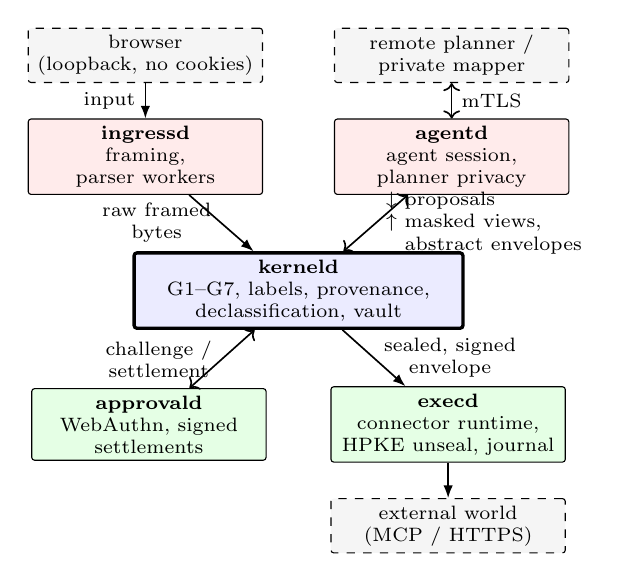
\begin{tikzpicture}[
  font=\scriptsize,
  node distance=4.5mm and 9mm,
  box/.style={draw,rounded corners=1pt,align=center,inner sep=2.5pt,minimum height=6mm,text width=28mm},
  untrusted/.style={box,fill=red!8},
  tcb/.style={box,fill=blue!8,very thick,text width=40mm},
  effect/.style={box,fill=green!10},
  ext/.style={box,dashed,fill=black!4},
  arr/.style={-{Latex[length=1.6mm]},semithick},
]
\node[untrusted] (ing) {\textbf{ingressd}\\framing, parser workers};
\node[untrusted,right=of ing] (ag) {\textbf{agentd}\\agent session,\\planner privacy};
\node[ext,above=of ing] (br) {browser\\(loopback, no cookies)};
\node[ext,above=of ag] (pl) {remote planner /\\private mapper};
\node[tcb] (k) at ($(ing)!0.5!(ag)+(0,-17mm)$) {\textbf{kerneld}\\G1--G7, labels, provenance,\\declassification, vault};
\node[effect] (ap) at ($(k)+(-19mm,-17mm)$) {\textbf{approvald}\\WebAuthn, signed\\settlements};
\node[effect] (ex) at ($(k)+(19mm,-17mm)$) {\textbf{execd}\\connector runtime,\\HPKE unseal, journal};
\node[ext,below=of ex] (world) {external world\\(MCP / HTTPS)};
\draw[arr] (br) -- node[left,pos=.5]{input} (ing);
\draw[arr,<->] (ag) -- node[right,pos=.5]{mTLS} (pl);
\draw[arr] (ing) -- node[left,pos=.5,align=center]{raw framed\\bytes} (k);
\draw[arr,<->] (ag) -- node[right,pos=.5,align=left]{$\downarrow$ proposals\\$\uparrow$ masked views,\\\phantom{$\uparrow$} abstract envelopes} (k);
\draw[arr,<->] (k) -- node[left,pos=.5,align=center]{challenge /\\settlement} (ap);
\draw[arr] (k) -- node[right,pos=.5,align=center]{sealed, signed\\envelope} (ex);
\draw[arr] (ex) -- (world);
\end{tikzpicture}
\caption{Process decomposition. Red components are untrusted by design;
the kernel is the TCB; green components hold effect or approval authority
but no policy authority. Every edge is a distinct mutually authenticated
Suite-1 channel with its own key pair, peer rule, and operation
vocabulary.}
\label{fig:arch}
\end{figure}

\subsection{Process decomposition}

\sys{} is a multi-daemon system (Figure~\ref{fig:arch}). Isolation is a
property of process boundaries, not module boundaries: a compromised role
cannot assume another's authority because it does not hold the other's keys
or socket credentials. The agent daemon \code{savana-agentd} owns agent
sessions and planner orchestration and is untrusted by design. All user
input enters through \code{savana-ingressd}, which frames bytes and runs
parsers in disposable one-job sandboxed workers. The kernel
\code{savana-kerneld} owns labels, provenance, declassification, the policy
gates, and the vault. \code{savana-approvald} owns WebAuthn credentials and
signed approval settlements. \code{savana-execd} owns connector credentials,
effect dispatch, and the durable execution journal. A trusted control shell
(``JARVIS'') can create tasks and read closed public status, but receives no
content and holds no data-plane key.

Seven inter-process edges exist, each with a distinct client key, server
key, peer rule, endpoint role and operation enumeration; there is no
JARVIS-to-kernel, JARVIS-to-executor, agent-to-executor or
ingress-to-executor data-plane edge. Every edge uses \emph{Suite-1}: a
fixed handshake prefix, ephemeral X25519, an Ed25519-signed handshake
transcript that binds both peers' process boot identifiers and the observed
OS peer identity, HKDF-SHA-256 traffic keys, mutual HMAC confirmation,
ChaCha20-Poly1305 records, and exactly one encrypted request and one
encrypted response per connection.

\subsection{Seven gates}

The kernel organizes enforcement as seven gates with a single Rust owner
each: G1 (Unicode normalization, indirect-injection policy, PII/credential
detection, tokenization), G2 (signed local extraction, closed grammar,
whitelist, abstract intent and slot construction), G3 (labels, provenance,
non-improving derivation, signed declassification rules), G4 (policy
$\times$ registry active set, closed ontology, attempt class, quota,
action-intent deduplication), G5 (manifest-bound internal validators only),
G6 (daemon-signed display and WebAuthn-backed single-use settlement), and G7
(fully bound durable action intent, atomic dispatch preparation, OS
effect-gate lease and fence epoch, execution nonce, result ingress,
reconciliation).

\subsection{The structural claim}

The agent holds no capability. Every capability-bearing operation is a
kernel state machine with its own verification path; the 25 agent-facing
kernel operations enumerate what an agent may \emph{ask for} and what each
request must \emph{prove}. This is the difference between ``the agent is
sandboxed'' and ``the agent has no authority to sandbox'': the kernel does
not filter the agent's actions, because the agent has no actions, only
requests.

\subsection{State ownership}

Each daemon's mutable security state is owned by one bounded owner thread.
Requests carry absolute deadlines and enter bounded queues; an owner panic,
an audit failure, an identity change, a detected rollback, or an uncertain
commit fail-stops the daemon. The agent and executor daemons additionally
hold a process-level \emph{effect gate}: a shared OS file lock on a fixed
inode plus an authenticated read-only ledger projection, taken across every
planner or effect transition and refused once the deployment helper has
begun a fenced cutover. This turns the race between ``a deployment is
switching generations'' and ``an effect is in flight'' into an OS-level
provable mutual exclusion.

% =====================================================================
\section{The Label Model}
\label{sec:labels}

\subsection{Dimensions}

Every value carries \lbl{\integ}{\conf}{\readers}{\effects}
(Table~\ref{tab:labels}). Integrity is a three-point total order in which
\emph{higher} means \emph{less} trusted, with join~$=\max$. Confidentiality
is a four-point lattice that is deliberately non-linear:
\textsf{PlannerAbstract} and \textsf{AgentMasked} are incomparable and join
to \textsf{VaultBound}. A value derived from something the external planner
may see and something the agent may see is therefore readable by
\emph{neither}; the safe outcome falls out of the algebra rather than a
special case. Readers and effects are closed bit sets over seven principals
and seven effects respectively.

\begin{table}[t]
\centering\footnotesize
\begin{tabularx}{\columnwidth}{@{}llX@{}}
\toprule
\textbf{Dim.} & \textbf{Structure} & \textbf{Values}\\
\midrule
$\integ$ & total order, $\join=\max$ &
  \textsf{KernelTrusted} $<$ \textsf{UserAuthorized} $<$ \textsf{ExternalUntrusted}\\
$\conf$ & lattice &
  \textsf{Public} $\sqsubseteq$ \{\textsf{PlannerAbstract}, \textsf{AgentMasked}\} $\sqsubseteq$ \textsf{VaultBound}\\
$\readers$ & bit set (7) &
  \textsc{kernel}, \textsc{agent}, \textsc{ingress}, \textsc{approval\_display}, \textsc{executor}, \textsc{external\_planner}, \textsc{external\_sink}\\
$\effects$ & bit set (7) &
  \READ, \textsc{create}, \textsc{update}, \textsc{delete}, \SEND, \textsc{execute}, \textsc{final\_release}\\
\bottomrule
\end{tabularx}
\caption{The four label dimensions.}
\label{tab:labels}
\end{table}

\subsection{Propagation narrows}

Derivation joins integrity and confidentiality upward and
\emph{intersects} readers and effects, then intersects effects with the
session's signed policy allowance. A derived value is readable by a subset
of every parent's readers and may cause a subset of every parent's effects.
This single choice makes declassification the only interesting operation in
the system: absent declassification, the reachable state space contains no
widening at all.

\subsection{The untrusted-effect ceiling}
\label{sec:ceiling}

Consider an agent that fetches a web page containing an attacker-supplied
address, combines it with a user-authorized document handle, and proposes
to send. Without further constraint the combined value's effect set derives
from the session-wide allowance and contains \SEND; the fabricated recipient
passes effect-based confinement. We call this \emph{effect laundering}:
authority acquired by combination.

\sys{} enforces
\[
\integ(v)=\textsf{ExternalUntrusted}\;\Rightarrow\;\effects(v)\subseteq\{\READ\}
\]
at construction, at derivation, and \emph{again after each join}
(Listing~\ref{lst:derive}). The re-application is the operative part: a
value combining a trusted and an untrusted parent becomes untrusted by the
integrity join and must therefore lose the authorizing effects its trusted
parent contributed. Without it the invariant holds pointwise at construction
and is violated by exactly the derivation that matters. Source
initialization is closed: signed policy constants begin
\textsf{KernelTrusted}; an approved ingress begins \textsf{UserAuthorized}
(approval authorizes \emph{use}, it does not assert truth); planner output,
tool results and values recovered after a crash are \emph{always}
\textsf{ExternalUntrusted}. The fact that the kernel performed a computation
is never evidence for an integrity upgrade.

\begin{lstlisting}[caption={Label derivation (abridged). The ceiling is re-applied after the join.},label={lst:derive},float=t]
pub const UNTRUSTED_CEILING: Effects = READ;

fn confined(i: Integrity, e: Effects) -> Effects {
    match i {
        ExternalUntrusted => e & UNTRUSTED_CEILING,
        _ => e,
    }
}

fn derive(parents: &[Label], allowed: Effects)
    -> Label {
    let mut d = parents[0];
    for p in &parents[1..] {
        d.int     = d.int.join(p.int);    // max
        d.conf    = d.conf.join(p.conf);  // join
        d.readers = d.readers & p.readers;
        d.effects = d.effects & p.effects;
    }
    d.effects = d.effects & allowed;
    // re-apply the ceiling AFTER the join
    d.effects = confined(d.int, d.effects);
    d
}
\end{lstlisting}

\subsection{Provenance}

Each value is accompanied by a provenance record naming its source kind
(one of eight: gated ingress, kernel extraction, policy constant, planner
output, tool result, derivation, kernel declassification, recovered
execution), its parents, its root evidence digests, its label, the
producing service identity, the durable run, the active state-manifest
digest, and an expiry. Bounds are compiled in (at most 256 parents and 64
root-evidence entries; bounded depth, node count and encoded size), so a
hostile lineage cannot exhaust the kernel. Parents from another run or
another manifest generation are refused, as is a parent whose value digest
does not match its record.

% =====================================================================
\section{Declassification}
\label{sec:declass}

\subsection{Five transitions, duties by recipient}

Because derivation only narrows, the only way a value's audience can grow
is an explicit declassification. \sys{} defines exactly five transitions
(Table~\ref{tab:transitions}). Each names a target
$(\conf,\readers)$ and a \emph{leak-gate duty}: what the content gate must
prove about the exact outgoing bytes before the transition may run.

\begin{table}[t]
\centering\scriptsize
\begin{tabularx}{\columnwidth}{@{}lXl@{}}
\toprule
\textbf{Transition} & \textbf{Target $(\conf,\readers)$} & \textbf{Gate duty}\\
\midrule
\textsf{MaskTokenizeAndLeakCheck} & (\textsf{AgentMasked}, \textsc{agent}) & blocklist $\wedge$ no PII\\
\textsf{BuildPlannerEnvelope} & (\textsf{PlannerAbstract}, \textsc{ext.\ planner}) & blocklist $\wedge$ no PII\\
\textsf{BuildApprovalDisplay} & (\textsf{AgentMasked}, \textsc{approval}) & blocklist\\
\textsf{BuildExecutionEnvelope}\,\{\emph{exec.}\} & (\textsf{VaultBound}, \textsc{executor}) & blocklist\\
\textsf{BuildFinalRelease}\,\{\emph{sink}\} & (\textsf{VaultBound}, \textsc{ext.\ sink}) & blocklist\\
\bottomrule
\end{tabularx}
\caption{The closed set of declassification transitions. The two that hand
a value to one recipient carry that recipient's identity digest inside the
variant.}
\label{tab:transitions}
\end{table}

The duty assignment follows \emph{who reads the result}, not how far
confidentiality drops---a distinction we believe is underappreciated. A
language model is the one recipient that cannot be trusted to hold personal
data without it becoming prompt context, training input, or an outbound
request; the two LLM-facing transitions must therefore be free of residual
PII. A human approver and an executor both need real values to perform
their function: nobody can meaningfully approve ``send
\code{[phone]} to \code{[email]}?'', and an executor with masked arguments
has nothing to act on. Masking those would not be a stricter gate but a
broken one. The blocklist---injected instructions---binds universally: no
recipient is entitled to those under any transition. A signed rule may
additionally raise a transition's duty floor but never lower it; the
constructor takes the stricter of the two.

\subsection{Exact-recipient binding}

For the executor and egress handoffs the recipient identity digest is
carried \emph{inside} the transition variant, so the transition cannot be
named without naming its reader, and the identity is bound into the
provenance node's evidence. A reader \emph{class} can express ``an external
sink may read this'', which cannot distinguish the release the user asked
for from a release to an attacker-chosen destination. At the egress boundary
that distinction is the entire security property. An all-zero identity is
refused.

\subsection{The checker computes its own evidence}
\label{sec:evidence}

The declassification constructor is private. It runs the gate and derives
the evidence digest from what the gate observed:
\begin{lstlisting}
let leak_gate_digest = enforce_for_declassification(
    value, transition.duty().strictest(rule.duty_floor()))?;
\end{lstlisting}
\code{leak_gate_digest} is deliberately not a parameter. Accepting it from
a caller would permit asserting a check the kernel cannot verify occurred,
at precisely the point where the kernel relinquishes a confidentiality
guarantee. The constructor further refuses records whose rule,
implementation, token-set or purpose digests are all zero: a record
``authorized by'' a rule that names nothing binds nothing.

\subsection{Signed rules}
\label{sec:rules}

A transition needs a referent for ``authorized''. \sys{} provides it with a
\emph{declassification rule set}: a canonically encoded, domain-separated,
hash-chained (sequence, previous signed digest) object signed by a key
authorized under a dedicated purpose---\textsf{DeclassificationAuthority}---of
the operational trust roots (\S\ref{sec:supply}). The rule set's signed
digest must equal a pin carried by the deployment manifest; a set that
verifies but does not match the pin is refused, because a
valid-but-unpinned rule set is exactly the substitution the pin exists to
prevent. Each rule binds a transition tag, a closed purpose (five values,
one per transition), an \emph{implementation digest}, a duty floor, an
optional sorted list of reader identities, an optional maximum consent
age, and a validity window nested inside the set's. Compiled hard limits
cap a set at 64 rules and a rule at 16 reader identities.

The public entry \code{declassify(...)} then checks, in order: the set is
within its window; a rule authorizes this (transition, purpose); the rule
is within its window; the rule's implementation digest equals the digest
\emph{compiled into the kernel} for that transition (so a rule cannot
authorize a transformation the running kernel does not implement); the
exact recipient, if any, is among the rule's reader identities; and, if the
rule demands consent, a verified final-release settlement is present and
validates---as a pure function---against the destination, token scope,
active manifest, issuance time and maximum age. Only then does the private
constructor run the gate and mint a node. For the final-release transition
an empty token scope is additionally refused.

Rule sets roll over atomically at runtime: a candidate is fully decoded,
verified against digest, signature, window and roots, then checked as a
valid successor of the active set under a write lock before a single
pointer swap; every failure leaves the old active set untouched. The
declassification trust root is also bound into the deployment transaction's
expected pre-state, so complete deployment trust includes the fourth chain.

\subsection{The handoff judgment}

Minting a node is necessary but not sufficient to cross a service boundary.
Every handoff consults \code{judge_handoff(transition, rules)}, which
returns \textsf{Admits}, \textsf{Refuses}, or \textsf{Unproven}. It is
\textsf{Unproven} unless the node's source kind is a kernel
declassification whose rule can be found in the active set; it
\textsf{Refuses} unless the node's confidentiality equals the transition's
target and its reader set contains the target readers, and---for exact
recipients---unless the identity appears both in the rule and in the node's
root evidence. Only \textsf{Admits} crosses. This is what makes the
$\conf$ and $\readers$ dimensions load-bearing rather than merely
propagated.

\subsection{Where the transitions run}

All five transitions are instantiated on the kernel's production paths:
masking at ingress (the agent's masked view carries the resulting node
digest, which is also bound into the vault record); planner-envelope
construction (the planner ticket carries the node digest); approval
displays for tool, release, ingress and connector-registration approvals
(the signed approval envelope carries the \emph{exact display bytes} and
the node digest, so the human approves precisely the bytes the gate saw);
execution envelopes; and final release. For the last two, a wrapper
enforces \emph{gate before durable prepare}: the durable-preparation
closure is unreachable if the gate refuses, so a refused handoff leaves the
dispatch state \textsf{Authorized} and reserved quota at zero. The durable
pre-seal digest binds the exact plaintext together with the node digest, so
recovery cannot alias the same bytes to a different provenance.

\subsection{One definition of ``sensitive''}
\label{sec:gate}

The masker at ingress and the verifier at declassification consume the
\emph{same} definition from a dedicated crate: a 21-pattern content
blocklist plus a 17-pattern PII table, where the PII span finder returns
the union of the pattern table and a blunter byte scanner, and a pattern-set
digest is folded into every gate digest. The two halves previously carried
separate definitions (\S\ref{sec:principles}). The patterns are ports of
Python regular expressions, and Python's \code{re} and Rust's linear
regex engine disagree on \code{\b}, \code{\s}, \code{\d} and
\code{\w}---the last in the bypass direction. Every character class is
therefore rewritten over character tables vendored from a pinned Unicode
version, word boundaries are rewritten as their two-sided literal
definition (which needs lookaround, hence a bounded backtracking engine),
and any engine error counts as a blocklist hit: adversarial input can only
cause the gate to over-block, never to miss. A differential corpus of 427
hand-constructed vectors in 17 behavioral groups and 6{,}000 fuzz vectors
mechanizes the one-way implication
$\mathit{masked}(x)\Rightarrow\mathit{gate\_passes}(\mathit{masked}(x))$.
Operationally this means routing the masking path through the gate costs no
false blocks today, and the day the halves drift the gate refuses and
ingress fails closed---a loud production error rather than a silent leak.

% =====================================================================
\section{Signed Authority and Durable Effects}
\label{sec:authority}

\subsection{The signed policy supply chain}
\label{sec:supply}

Nothing in \sys{} is configured; everything is signed. An installer/MDM key
signs \emph{operational trust-root sets}: canonically encoded,
domain-separated, hash-chained objects whose members carry one of five
purposes (deployment authorization, rollback authorization, installation
activation, installer/MDM, declassification authority), each with a key
epoch and a validity window nested inside the set's; members are sorted
and deduplicated and the member-set binding digest is recomputed at decode.
Above the roots sit signed deployment manifests and claims (release
identity, binary and projection pins, the declassification rule-set pin), a
signed tool-descriptor registry whose publisher key is authenticated by the
active state manifest, and the executor material (identity, key id, seal
public key, connector-registry digest) bound into every dispatch through an
effect-gate lease.

Three disciplines recur across every signed object and constitute, in our
experience, a reusable house style for security-critical Rust:
\begin{enumerate}
\item \textbf{Possession implies verification.} Verified types have
  private fields and a single verifying constructor. Holding the value is
  the proof; downstream code cannot forget to re-check because there is
  nothing to re-check. Negative API contracts (``this identity exposes no
  seed'', ``this handshake state cannot be cloned'') are enforced as
  \code{compile_fail} documentation tests.
\item \textbf{Canonical re-encode equality.} Decode, re-encode, compare to
  the input bytes. Any non-canonical encoding---a mutated byte, an
  alternate integer width, an indefinite-length container---is refused.
  The workspace uses 461 distinct NUL-terminated domain-separation strings
  to prevent cross-protocol signature reuse.
\item \textbf{Chain, don't patch.} Revocation is expressed by publishing a
  successor; predecessor validation enforces sequence continuity, digest
  linkage and family identity. There are no tombstones and no partial
  updates.
\end{enumerate}

\subsection{Deployment transactions}

Policy, registries, models, sandbox profiles, service identities and
binaries activate as one signed restart transaction. The deployment core
implements a dual-slot signed ledger; a ``highest-ever'' vector over 29
closed security domains that provides anti-rollback across generations; a
25-step transaction head with typed evidence references; a head-first,
ledger-compare-and-swap transition store that authenticates head ancestry
before progress and never selects an orphan by time or chain length; a
fixed-inode cross-process mutex; and recovery of the one crash window
between a durable successor slot and the native monotonic-counter advance.
Compaction of an aborted transaction requires a signed evidence checkpoint
carried on a hash-chained evidence envelope. Missing, expired, mis-signed or
unpinned material yields a kernel that runs and refuses; the startup matrix
requires that corrupt bootstrap material leaves \emph{no socket bound}.

\subsection{Human approval: two ceremonies}

Approval is a G6 round trip. The kernel mints a challenge-bearing,
principal-bound approval envelope carrying the exact gated display bytes
and their declassification node digest, signs it, and pairs it with a UI
authentication envelope. The approval service returns no display until a
fresh WebAuthn \emph{display-authentication} ceremony has established an
in-memory, tab-bound approval session; the user then performs a second,
distinct WebAuthn \emph{decision} ceremony. The two use different signed
types, domains, challenges, nonces and one-use states: display
authentication can never approve, and a decision assertion can never create
or resume a display session. Settlements are signed under per-purpose keys
(UI authentication, ingress, tool execution, final release, connector
registration), so a settlement for one purpose cannot verify as another.
The kernel verifies a settlement against the settlement key, installation
identifier, active manifest digest, deployment generation, envelope digest,
principal and challenge, and consumes it once.

\subsection{Journal before effect}
\label{sec:pipeline}

Before writing a single byte toward an executor, the kernel commits one
atomic effect-preparation transaction. It verifies exactly one closed
dispatch subject (a tool execution binding the durable action intent,
descriptor, complete argument binding, provenance set and attempt class; or
a final release binding a distinct release identifier, vault segment,
evidence, token set, destination projection and release policy); consumes
the ticket and the settlement where required; moves quota from available to
reserved in a branch-typed bucket; locks every field of the subject plus
the exact executor and active manifest; creates the \emph{sole} execution
nonce; stores the HPKE-sealed subject-specific envelope, an AEAD-sealed
exact-replay capsule and a \textsf{Prepared} journal entry; and binds the
dispatch to the current effect-fence epoch. Either every kernel-owned item
becomes durable or none does; there is no fictitious cross-daemon ACID.

The executor's journal is the durable truth at the external-byte boundary:
it fsyncs a receipt-free \textsf{ProviderAttemptPrepared}, then signs and
stores an \textsf{EffectStarted} receipt, and only then may emit the first
provider byte; the bounded provider response is encrypted and fsynced
before any codec sees it; a final release additionally prepares audit
evidence before the signed final receipt. Receipts and journal records form
a directed hash DAG. On the kernel side a recovery state machine classifies
each dispatch as prepared, dispatching, effect-started, completion
committed, failed-with-no-effect, or indeterminate. Only a \emph{proven}
no-effect failure may be re-planned; an indeterminate effect and
``effect succeeded, output quarantined'' are never retried automatically.
The provenance source kind \textsf{RecoveredExecution} exists so that a
value produced by an action whose outcome was learned after a crash is
distinguishable from a fresh result and carries \textsf{ExternalUntrusted}
integrity like any other external result.

% =====================================================================
\section{Beyond Values: Shape, Intent, and Connectors}
\label{sec:beyond}

\subsection{Planner privacy}

Value masking protects the first of three leakage layers. A system that
uses a remote planning model also leaks the plan's \emph{shape} (how many
steps, which capability classes, in what dataflow order, to which kinds of
sink) and the user's \emph{intent} (which lives in the task's verbs, not in
values a masker redacts). \sys{} splits planning into three agent-side
stages without changing the kernel:
\begin{enumerate}
\item a \emph{mapper} model, inside the user's intent trust domain,
  receives a nonce-free intent projection and the intersection of active
  tools with a local semantic catalog, and produces a structural graph;
\item a \emph{planner} model, which may be third-party, receives only that
  graph: nodes with fresh per-run identifiers, coarse roles
  (\textsc{source}/\textsc{transform}/\textsc{sink}), coarse effect classes,
  edges, and a fixed dataflow-ordering goal (at most 256 nodes and 4{,}096
  edges);
\item a \emph{deterministic decoder} maps the ordered plan back to tool
  classes and a local nonce. This stage must not be a model: a decoder that
  hallucinates picks a different tool, which is a security defect, not an
  accuracy problem. The kernel's existing class resolution then authorizes
  as before.
\end{enumerate}
Intent exposure is a single explicit knob---a deployment ceiling
(\textsf{PrivateOnly} or \textsf{UserMayUseThirdParty}) and a per-task user
choice that fails safe to private. TLS identity is separated from network
routing: endpoint hosts are used only for SNI and certificate matching,
while a signed, bounded, sorted connect-address list is the only routing
input; there is no DNS fallback, and on Linux the base service denies all IP
traffic while a root-owned generated drop-in permits exactly the measured
addresses. The design states its information-theoretic floor up front:
whoever produces a plan learns its shape. Shape can be de-semanticized; it
cannot be hidden from the planner outright.

\subsection{Connector registration through the signed channel}

Adding a tool to a running installation must not weaken the rule that
registration verbs exist only in signed channels. \sys{} makes the
connector registry a hash-chained state whose genesis digest and update
authority are pinned by the deployment channel: self-service extends the
chain and can never escape it. The kernel and the executor verify the chain
independently and converge; divergent heads fail dispatch exactly as a
digest mismatch does today. Connectors have tiers
(\textsf{DeploymentShipped}, \textsf{UserRegistered}), and a tier is a
capability ceiling: a user-registered connector is a tool surface and can
structurally never become an egress sink; user-tier connectors are
restricted to a host allowlist and their own identifier namespace, and each
descriptor signs its structural role for the planner catalog. A proposal
can only originate from an authenticated agent browser tab, is bound to a
one-use kernel authorization covering the exact descriptor bytes, current
registry head, session, principal, task, run, origin, caller boot, manifest
and generation, and is settled by a distinct-purpose approval whose display
shows the complete descriptor, transport identity, and every tool's
semantics---released, like every other display, through a real
declassification.

% =====================================================================
\section{Implementation}
\label{sec:impl}

\sys{} is implemented in Rust (edition 2021, toolchain pinned) with
\code{unsafe_code = "forbid"} at the workspace level; only the platform
crate downgrades to \code{deny} and re-enables unsafe code locally in four
audited native-boundary modules (systemd descriptor takeover, the Linux
Landlock/seccomp launcher, macOS Security.framework FFI, and the macOS
Seatbelt launcher). Table~\ref{tab:impl} gives the breakdown measured at
the commit this paper describes. Eleven crates form a production core
frozen by a SHA-256 manifest of 164 files; the manifest check, and an
adversarial test of the checker itself, are the first CI steps.

\begin{table}[t]
\centering\footnotesize
\begin{tabularx}{\columnwidth}{@{}lrX@{}}
\toprule
\textbf{Crate} & \textbf{LOC} & \textbf{Role}\\
\midrule
policy-core & 85{,}589 & labels, provenance, rules, engine, deployment\\
kerneld & 62{,}857 & kernel daemon, authorities, data plane, recovery\\
kernel-protocol & 43{,}644 & closed wire vocabulary, Suite-1, CBOR\\
agentd & 22{,}806 & agent sessions, planner privacy\\
execd & 17{,}791 & connector runtime, journal, sandboxed workers\\
approvald & 12{,}711 & WebAuthn, settlements\\
client & 8{,}933 & Rust SDK state machine\\
ingressd & 8{,}594 & framing, parser workers\\
platform-identity & 4{,}993 & native measurement, sandboxes\\
vault & 4{,}004 & sealed custody, release material\\
leak-gate & 1{,}745 & the one definition of ``sensitive''\\
input-runtime & 1{,}466 & G1/G2\\
others & 20{,}482 & Python binding, release receiver, legacy NER, tooling\\
\midrule
\textbf{Total} & \textbf{295{,}615} & 16 crates, 11 frozen\\
\bottomrule
\end{tabularx}
\caption{Implementation size (lines of Rust). Application-side
integration adds 6{,}622 lines of Python and 3{,}565 lines of TypeScript.}
\label{tab:impl}
\end{table}

\paragraph{Cryptography.} Ed25519 signatures with weak-key rejection;
SHA-256 domain-separated digests; X25519 with HKDF and
ChaCha20-Poly1305 or AES-GCM for sealed envelopes and durable records;
canonical CBOR~\cite{rfc8949}; entropy from the OS with explicit zero
checks on generated nonces. All dependency versions are pinned exactly.

\paragraph{Sandboxing.} Parser and connector-codec workers are one-job
child processes over anonymous inherited pipes with cleared environments
and bounded transcripts. On Linux the launcher applies
Landlock~\cite{landlock} path rules, a seccomp-BPF filter with a
kill-process default, descriptor closure and resource limits; on macOS a
deny-default Seatbelt profile with a parent supervisor that terminates a
child above its measured memory footprint. A missing or changed sandbox
wrapper or profile fails closed.

\paragraph{Application integration.} A client SDK exposes exactly three
loopback services (agent, ingress, approval), fifteen business methods and
eighteen product types; handles expose no raw bytes and cannot be retagged,
and the bounded autonomous loop re-plans only after a proven no-effect
failure. A production integration into an existing agent framework
registers one provider, one model and one harness, zero framework tools and
zero MCP servers; every tool call, including read-only calls, and the final
release each consume a fresh approval obtained through a trusted product UI
over an inherited broker descriptor, and only bytes delivered by the
executor over a pinned mutual-TLS receiver with a durable single-flight
reservation can become an assistant reply. \todo{decide whether to name the
framework in the camera-ready.}

\paragraph{Testing assets.} The workspace contains 1{,}568 Rust test
functions in 163 unit-test modules and 92 integration-test files, 65
\code{compile_fail} documentation tests, the 6{,}427-vector gate corpus, an
adversarial policy matrix (signature forgery, equivocation,
expiry-versus-signature refusal ordering, replay across boots and
rollovers), a crash matrix over the durable pipeline, a startup matrix over
corrupt and partial installation material, an 821-line negative matrix for
declassification rule sets, and worker-isolation tests for both worker
kinds.

% =====================================================================
\section{Evaluation}
\label{sec:eval}

\pending{This section is a skeleton. Research questions, methodology and
table shells are fixed; every number is to be measured. Nothing below
should be read as a result.}

\subsection{Research questions}

\begin{description}[style=nextline,font=\bfseries]
\item[RQ1 Structural impossibility.] For a corpus of published prompt-injection attacks against tool-using agents, which attack classes become \emph{structurally impossible} under the label model (as opposed to \emph{detected}), and which remain?
\item[RQ2 Gate soundness and agreement.] Does the shared content gate satisfy $\mathit{masked}(x)\Rightarrow\mathit{gate\_passes}(\mathit{masked}(x))$ beyond the shipped corpus, and what are its recall and over-blocking rates on labeled PII data?
\item[RQ3 Cost.] What do labels, provenance, the gate, signed rules and the journal-before-effect pipeline cost in latency, throughput and memory relative to an ungated baseline?
\item[RQ4 Crash and rollover consistency.] Under adversarially timed crashes and policy rollovers, does the system ever produce a duplicate effect, lose an effect it reported, or admit a value whose provenance was not recorded?
\item[RQ5 Utility.] How often does the closed structural planning pipeline produce a plan the kernel authorizes, compared with sending the full envelope to the planner?
\end{description}

\subsection{Experimental setup}

\todo{hardware; OS and kernel versions (Landlock availability); Rust
toolchain; model endpoints used for mapper and planner; connector set;
baseline configuration (same daemons with gate, rules and journal disabled,
or an unmodified framework agent); number of trials; statistical treatment.}

\subsection{RQ1: Security against a published attack corpus}

\todo{Attack sources: AgentDojo~\cite{debenedetti2024agentdojo},
InjecAgent~\cite{zhan2024injecagent}, and hand-written attacks targeting
each of the five transitions and the connector-registration path. For each
attack: the label state at the point of refusal, whether refusal is
structural (no request exists that could succeed) or gated (a request
exists and the gate refused), and the refusal's stable error code.}

\begin{table}[h]
\centering\footnotesize
\begin{tabularx}{\columnwidth}{@{}Xrrrr@{}}
\toprule
\textbf{Attack class} & \textbf{\#} & \textbf{Struct.} & \textbf{Gated} & \textbf{Succ.}\\
\midrule
Data exfiltration via tool argument & \tbd & \tbd & \tbd & \tbd\\
Unauthorized effect (send/execute) & \tbd & \tbd & \tbd & \tbd\\
Approval-display manipulation & \tbd & \tbd & \tbd & \tbd\\
Connector injection & \tbd & \tbd & \tbd & \tbd\\
Planner-output authority claim & \tbd & \tbd & \tbd & \tbd\\
\midrule
Total & \tbd & \tbd & \tbd & \tbd\\
\bottomrule
\end{tabularx}
\caption{\todo{Outcome of each attack class under \sys{}. ``Structural''
means no protocol request could have caused the effect; ``gated'' means a
runtime check refused it.}}
\label{tab:attacks}
\end{table}

\subsection{RQ2: Gate agreement, recall and over-blocking}

\todo{Extend the differential corpus with (i) a labeled PII corpus in the
languages the deployment supports and (ii) generated adversarial encodings
(homoglyphs, zero-width joiners, NFKC-divergent forms). Report recall per
PII class, over-blocking rate on benign text, and the agreement rate between
masker and verifier.}

\begin{table}[h]
\centering\footnotesize
\begin{tabularx}{\columnwidth}{@{}Xrrr@{}}
\toprule
\textbf{Class} & \textbf{Recall} & \textbf{Over-block} & \textbf{Agreement}\\
\midrule
Credential & \tbd & \tbd & \tbd\\
Personal data & \tbd & \tbd & \tbd\\
Protected reference & \tbd & \tbd & \tbd\\
Injected instruction (blocklist) & \tbd & \tbd & \tbd\\
\bottomrule
\end{tabularx}
\caption{\todo{Content-gate quality.}}
\label{tab:gate}
\end{table}

\subsection{RQ3: Cost}

\todo{Micro-benchmarks: gate cost per transition as a function of input
size; label derivation and provenance-node construction as a function of
parent count and DAG depth; rule-set verification and rollover. Macro-benchmarks:
end-to-end latency of ingest $\rightarrow$ plan $\rightarrow$ tool call
$\rightarrow$ release versus the baseline; throughput under concurrent
sessions; memory of provenance state per session.}

\begin{table}[h]
\centering\footnotesize
\begin{tabularx}{\columnwidth}{@{}Xrrr@{}}
\toprule
\textbf{Component} & \textbf{Median} & \textbf{p99} & \textbf{vs.\ base}\\
\midrule
Gate, blocklist-only (8\,KiB) & \tbd & \tbd & --\\
Gate, blocklist $\wedge$ PII (8\,KiB) & \tbd & \tbd & --\\
Derivation (256 parents) & \tbd & \tbd & --\\
Effect-preparation transaction & \tbd & \tbd & \tbd\\
End-to-end tool call & \tbd & \tbd & \tbd\\
End-to-end final release & \tbd & \tbd & \tbd\\
\bottomrule
\end{tabularx}
\caption{\todo{Latency (ms) and overhead.}}
\label{tab:perf}
\end{table}

\subsection{RQ4: Crash and rollover consistency}

\todo{Fault injection at every journal boundary named in
\S\ref{sec:pipeline} and at every step of a rule-set and policy rollover;
oracle: the executor journal, the kernel WAL and the vault release state
must reconcile to exactly one of the six recovery states with no duplicate
nonce. Report trials, injected points, and violations (expected: 0).}

\subsection{RQ5: Planning utility under privacy}

\todo{Task suite; success rate and authorized-plan rate for (a) full
envelope to planner, (b) private mapper + third-party structural planner,
(c) private-only; number of re-plans; qualitative failure analysis.}

\subsection{Case study}

\todo{One end-to-end trace of an injected agent attempting exfiltration:
the fetched content's label, the derivation that would have laundered
\SEND, the ceiling re-application, the refused handoff judgment, and the
audit record. One figure.}

% =====================================================================
\section{Discussion and Limitations}
\label{sec:discussion}

\paragraph{Enforced versus by construction.} A claim that a system
enforces a property is meaningful only if the system distinguishes
enforcement from coincidence. An earlier revision of \sys{} had the
declassification constructor fully built and tested but reachable from no
production path; the masked agent view and the planner envelope were safe
\emph{by construction}---the masker provably satisfied the gate over the
corpus, and the envelope was structurally abstract---but not \emph{by
enforcement}, since nothing would have noticed if the two implementations
had stopped agreeing. The current design closes that gap on all five paths.
We regard the distinction as one the literature should insist on.

\paragraph{Platform root of trust.} The production deployment path requires
a non-exportable platform keystore adapter and a hardware-backed monotonic
rollback authority. The sealed platform boundary currently reports that
authority as unavailable, and the deployment binaries deliberately exit
unavailable rather than run with file-backed substitutes. Until a target
adapter is compiled and attested, the system does not claim platform or
product completeness, and development deployments use explicitly gated
file-backed authorities that release builds refuse at compile time.

\paragraph{Detection recall.} The content gate is deterministic
(patterns and a byte scanner); its recall is below a measured NER model. The
failure direction is safe, but recall is not at the design's intended
level. The rule surface anticipates a measured worker that may
\emph{propose} spans: proposals only add masking, the deterministic union
stays the floor, the gate remains the sole decider, and the worker's output
is \textsf{ExternalUntrusted}. Because the masking contract is pinned by the
pattern-set digest, a recall improvement is a visible signed policy change
rather than silent drift.

\paragraph{What the planner still learns.} Under remote structural
planning the planner sees node count, coarse roles and topology. Hiding
topology requires local planning or template selection.

\paragraph{Assurance.} \sys{} has had no third-party audit or penetration
test, and no formal verification: the invariants of \S\ref{sec:ceiling} and
\S\ref{sec:evidence} are stated in prose and enforced by construction.
Mechanizing the label algebra in a proof assistant or with refinement types
is the natural next step. Several integration suites also assume an
unprivileged test runner and a kernel with Landlock, which makes them
environment-sensitive.

\paragraph{Human factors.} Two WebAuthn ceremonies per approval and one
approval per tool call are deliberate, and they cost attention. Whether
users habituate, and whether the exact-bytes display is legible enough to
carry the decision it is asked to carry, are empirical questions we do not
answer here. \todo{consider a small user study or defer explicitly.}

% =====================================================================
\section{Related Work}
\label{sec:related}

\paragraph{Information-flow control.} \sys{}'s label model descends from
lattice IFC~\cite{denning1976}, the decentralized label
model~\cite{myers1997}, and IFC operating systems---Asbestos, HiStar and
Flume~\cite{efstathopoulos2005,zeldovich2006,krohn2007}---which established
process-granularity flow control with declassification as an explicit
privileged operation, as well as language-level dynamic IFC such as
LIO~\cite{stefan2011lio}. Our contribution is not the lattice but its
application: readers are system roles and named external identities rather
than users; declassification duties are assigned by recipient
trustworthiness, specifically by whether the recipient is a language model;
and the recipient identity is bound into the transition.

\paragraph{LLM agent security.} CaMeL~\cite{debenedetti2025camel}
established control/data-flow separation with capabilities for LLM agents
and demonstrated it at prototype scale; FIDES~\cite{costa2025fides} applies
IFC labels to agent planning with a focus on confidentiality;
IsolateGPT~\cite{wu2025isolategpt} isolates applications within an agent;
Progent~\cite{shi2025progent} adds programmable privilege control over tool
calls; and design-pattern surveys~\cite{beurerkellner2025patterns,willison2025trifecta}
catalog structural defenses. \sys{} shares the architectural thesis and
differs in engineering completeness---signed supply chain, durability and
crash recovery, real transports, adversarial matrices---and in addressing
shape and intent leakage. Detection- and training-based
defenses~\cite{wallace2024hierarchy,hines2024spotlighting,chen2025struq,chen2025secalign}
and formal benchmarks~\cite{liu2024formalizing,debenedetti2024agentdojo,zhan2024injecagent}
are complementary: they operate inside the boundary \sys{} relocates, and
they supply the corpora \S\ref{sec:eval} evaluates against.

\paragraph{Supply chain and confidential computing.} The manifest,
trust-root and sealed-envelope discipline draws on binary transparency and
in-toto-style supply-chain integrity~\cite{torresarias2019intoto}, applied
to \emph{policy} rather than to artifacts, and on HPKE~\cite{rfc9180} and
WebAuthn~\cite{webauthn2} for sealing and human authentication.

% =====================================================================
\section{Conclusion}
\label{sec:conclusion}

Prompt injection is unsolvable at the layer where it is usually attacked,
because the model is both the interpreter of untrusted input and the holder
of authority. \sys{} separates these: the model proposes, the kernel
disposes, values carry labels that only narrow, and the single widening
operation is rule-authorized, gate-verified, recipient-bound and recorded.
We described the architecture, the supply chain that makes it operable, the
durable pipeline that makes it honest about crashes, the privacy layers
above values, and the design principles we extracted from our own defects.
\todo{one sentence on the evaluation.}

% =====================================================================
\section*{Ethics Considerations}

This work builds a defensive system and evaluates it against attack
techniques that are already public. \todo{Confirm before submission:} the
planned evaluation uses published benchmark attacks and synthetic
documents; no human subjects, personal data of real individuals, or live
third-party services are involved beyond the model endpoints named in
\S\ref{sec:eval}; the PII corpus used for RQ2 is synthetic or
appropriately licensed. The content blocklist contains patterns for
harmful-content categories; it is reproduced from an existing production
filter and is used only to \emph{refuse} content. We identified no
stakeholder who is harmed by the publication of this design.

\section*{Open Science}

\todo{Confirm artifact plan.} The complete implementation described in
this paper, including the differential corpus, the adversarial and crash
matrices, the deployment units, and the evaluation harness for
\S\ref{sec:eval}, will be made available as a public repository at a
commit-pinned URL, together with the data and scripts needed to reproduce
every table. The source is currently under a proprietary license; a release
under an OSI-approved license is planned before artifact evaluation.
Model endpoints used in the evaluation will be documented by provider,
model identifier and date.

\ifanonymous\else
\section*{Acknowledgments}
\todo{acknowledgments}
\fi

\bibliographystyle{plain}
\bibliography{references}

% =====================================================================
\appendix

\section{Kernel Operation Vocabulary}
\label{app:ops}

The agent-facing kernel role accepts 25 operations
(health, claim/close session, prepare new and follow-up ingress, session
status, prepare planner call, commit planner value, derive value, propose /
evaluate / authorize tool call, dispatch execution, execution status, read
agent view, prepare / authorize / dispatch release, release status, revoke
vault, prepare and authenticate agent UI, kernel task status and cancel,
resume committed authentication); the ingress-facing role 12; the executor
role 5; the control shell 4; and connector control 2. Authenticated
requests cannot select handlers or cross roles; the startup
route-completeness gate proves one closed handler per operation before the
kernel publishes readiness.

\section{Design Principles from Defects}
\label{sec:principles}

Each principle below was extracted from a defect found and fixed during
the system's own security review. We report them because negative results
of this kind are the transferable part of systems-security work.

\begin{description}[style=nextline,font=\bfseries]
\item[Untrusted integrity must cap authority, transitively.]
\emph{Defect:} untrusted values inherited authorizing effects from the
session allowance, and derivations mixing trusted and untrusted parents kept
the trusted parent's effects. \emph{Fix:} the post-join ceiling
(\S\ref{sec:ceiling}).
\item[The checker computes its own evidence.]
\emph{Defect:} the declassification record accepted the gate digest as a
parameter. \emph{Fix:} compute it inside the constructor
(\S\ref{sec:evidence}).
\item[A record that names nothing binds nothing.]
\emph{Defect:} records with all-zero rule, implementation, purpose and
recipient digests were constructible. \emph{Fix:} zero refusal on every
binding digest. A permissive construction path adjacent to a strict one is
the one attackers will use.
\item[One definition of the predicate, mechanized.]
\emph{Defect:} the masker and the verifier consulted different definitions
of ``sensitive''. \emph{Fix:} one crate, one union, a digest in every gate
record, and a differential corpus (\S\ref{sec:gate}). Code review does not
detect drift; drift is silent.
\item[Gate before durable prepare.]
\emph{Defect:} a refused gate could leave a reserved quota and a prepared
dispatch behind. \emph{Fix:} an ordering boundary in which the durable
closure is unreachable on refusal.
\item[Consent is a pure check, consumed durably.]
\emph{Defect:} in-memory single-use consumption of a release settlement
made a blocked attempt consume the user's consent and a crash lose it.
\emph{Fix:} pure validation plus one-use enforcement inside the durable
dispatch preparation, with exact-replay acceptance only when release
binding, settlement digest, ticket, sealed payload digest and authority all
match.
\item[Absence of a symbol is not absence of a pipeline.]
\emph{Methodological:} an audit concluded from the absence of callers to
the declassification constructor that no egress path existed. It existed
and was elaborate; it simply bypassed the provenance system. Audit by data
flow, not by symbol reference.
\end{description}

\end{document}
